\documentclass{article}

\usepackage{graphicx}
\usepackage{tikz}
\usepackage{tikzsymbols}
\usetikzlibrary{calc,patterns,shapes.geometric}
\pagestyle{empty}
\usepackage[margin=0pt]{geometry}
\geometry{papersize={14in,12in}}

\def\centerarc[#1](#2)(#3:#4:#5){\draw[#1] ($(#2)+({#5*cos(#3)},{#5*sin(#3)})$) arc (#3:#4:#5);}

\begin{document}
	\begin{figure}
		\centering
		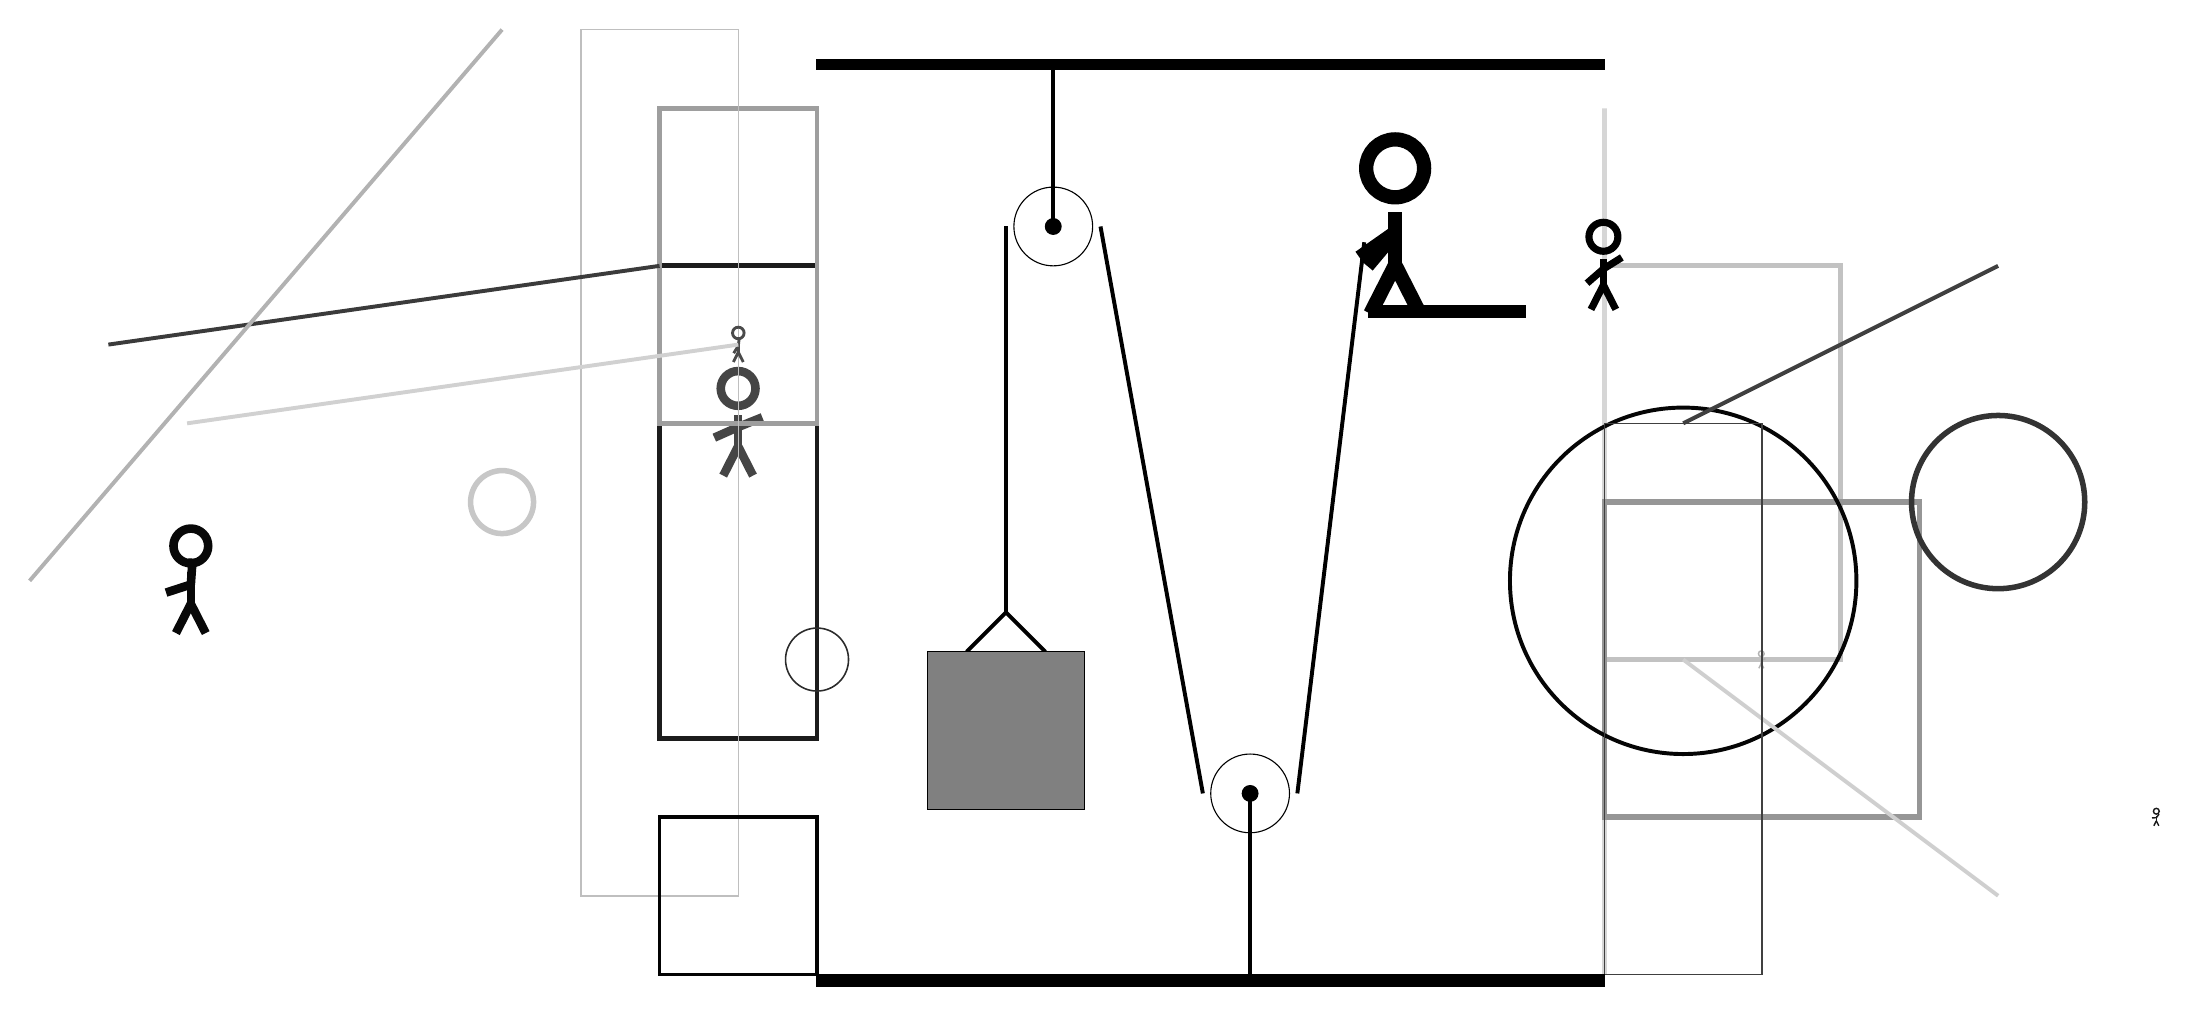
\begin{tikzpicture}
			%%%%% START %%%%%
			
			\draw[fill=black] (-2, 11.5) rectangle (8, 11.625);
			
			\draw (3.5, 2.3) circle (0.5);
			\draw[fill=black] (3.5, 2.3) circle (0.1);
			\draw[line width=0.5mm] (3.5, 2.3) -- (3.5, 0);
			
			\draw (1, 9.5) circle (0.5);
			\draw[fill=black] (1, 9.5) circle (0.1);
			\draw[line width=0.5mm] (1, 11.5) -- (1, 9.5);
			
			\draw[line width=0.5mm](-0.1, 4.1) --  (0.4, 4.6) -- (0.9, 4.1);
			\draw[fill=black!50] (-0.6, 4.1) rectangle (1.4, 2.1);
			
			\draw[line width=0.6mm, color=black!24] (8, 9) rectangle (11, 4);
			
			\draw[line width=0.7mm, color=black!16] (8, 0) rectangle (8, 11);
			\node[line width=0.3mm, color=black!73] at (-3, 7) {\Strichmaxerl[6][24][22]};
			\draw[line width=0.6mm, color=black!89] (-2, 3) rectangle (-4, 9);
			
			\draw[line width=0.2mm, color=black!27] (-4, 2) rectangle (-4, 2);
			\node[line width=0.6mm, color=black!30] at (10, 4) {\Strichmaxerl[1][86][19]};
			\draw[line width=0.6mm, color=black!38] (-4, 11) rectangle (-2, 7);
			
			\draw[line width=0.7mm, color=black!41] (8, 2) rectangle (12, 6);
			\draw [line width=0.2mm, color=black!83](-2, 4) circle (0.4);
			\draw [line width=0.7mm, color=black!22](-6, 6) circle (0.4);
			\node[line width=0.4mm, color=black!100] at (8, 9) {\Strichmaxerl[5][41][32]};
			\draw[line width=0.2mm, color=black!25] (-3, 1) rectangle (-5, 12);
			\draw [line width=0.5mm, color=black!98](9, 5) circle (2.2);
			
			\node[line width=0.5mm, color=black!97] at (-10, 5) {\Strichmaxerl[6][18][86]};
			\draw[line width=0.5mm, color=black!19](13, 1) -- (9, 4);
			\draw [line width=0.7mm, color=black!80](13, 6) circle (1.1);
			\draw[line width=0.3mm, color=black!88] (10, 7) rectangle (10, 5);
			\node[line width=0.7mm, color=black!90] at (15, 2) {\Strichmaxerl[1][4][52]};
			\node[line width=0.2mm, color=black!71] at (-3, 8) {\Strichmaxerl[2][58][83]};
			\draw[line width=0.5mm, color=black!18](-3, 8) -- (-10, 7);
			\draw[line width=0.5mm, color=black!75](9, 7) -- (13, 9);
			
			\draw[line width=0.5mm, color=black!77](-4, 9) -- (-11, 8);
			\draw[line width=0.2mm, color=black!75] (10, 0) rectangle (8, 7);
			\draw[line width=0.4mm, color=black!99] (-4, 0) rectangle (-2, 2);
			\draw[line width=0.5mm, color=black!30](-6, 12) -- (-12, 5);
			
			\draw[line width=0.5mm](0.4, 9.5) -- (0.4, 4.6);
			\centerarc[line width=0.5mm](1, 9.5)(180:0:0.6)
			\draw[line width=0.5mm](1.6, 9.5) -- (2.9, 2.3);
			\centerarc[line width=0.5mm](3.5, 2.3)(180:360:0.6)
			\draw[line width=0.5mm](4.1, 2.3) -- (4.95, 9.3);
			
			\node at (5.3, 9.5) {\Strichmaxerl[10][35][-130]};
			\draw[fill=black] (5, 8.5) rectangle (7, 8.35);
			
			\draw[fill=black] (-2, 0) rectangle (8, -0.15);
			
			%%%%% END %%%%%
		\end{tikzpicture}
	\end{figure}	
\end{document}